\documentclass[conference]{IEEEtran}
\IEEEoverridecommandlockouts

\usepackage{cite}
\usepackage{amsmath}
% Times-style fonts for XeTeX/Tectonic (IEEE uses Times)
\usepackage{fontspec}
\usepackage{unicode-math}
\setmainfont{texgyretermes}[Extension=.otf, UprightFont=*-regular, BoldFont=*-bold, ItalicFont=*-italic, BoldItalicFont=*-bolditalic]
\setmathfont{texgyretermes-math.otf}
\usepackage{algorithm}
\usepackage{algpseudocode}
\usepackage{graphicx}
\usepackage{textcomp}
\usepackage{xcolor}
\usepackage{booktabs}
\usepackage{multirow}
\usepackage{url}
\usepackage{tikz}
\usetikzlibrary{positioning,arrows.meta,fit,calc}
\usepackage{pgfplots}
\pgfplotsset{compat=1.17}

% Force a line break between author rows (2 x 2 grid)
\makeatletter
\newcommand{\linebreakand}{%
  \end{@IEEEauthorhalign}
  \hfill\mbox{}\par
  \mbox{}\hfill\begin{@IEEEauthorhalign}
}
\makeatother

\begin{document}

\title{Traffic-Aware Public Transit Route Optimization for Pune Using Classical Shortest-Path Algorithms and Interpretable Congestion Prediction}

\author{
\IEEEauthorblockN{Devang R. Patil}
\IEEEauthorblockA{PRN: 1251070841\\
Vishwakarma Institute of Technology\\
Pune, India\\
devang.1251070841@vit.edu}
\and
\IEEEauthorblockN{Chaitanya Ravi Patil}
\IEEEauthorblockA{PRN: 1251070797\\
Vishwakarma Institute of Technology\\
Pune, India\\
chaitanya.1251070797@vit.edu}
\linebreakand
\IEEEauthorblockN{Disha H. Patil}
\IEEEauthorblockA{PRN: 1251070923\\
Vishwakarma Institute of Technology\\
Pune, India\\
disha.1251070923@vit.edu}
\and
\IEEEauthorblockN{Divya Yogesh Patil}
\IEEEauthorblockA{PRN: 1251070077\\
Vishwakarma Institute of Technology\\
Pune, India\\
divya.1251070077@vit.edu}
}

\maketitle

% =====================================================================
\begin{abstract}
Commuters in Pune experience large differences in travel time between
peak and off-peak hours, yet most route planners used in coursework rank
routes purely by distance. This paper presents a transit route optimizer
for 24 major Pune Mahanagar Parivahan Mahamandal Ltd. (PMPML) hubs and
38 road corridors, written from scratch in C++17. Three classical
shortest-path paradigms are implemented and benchmarked side by side:
Dijkstra's algorithm (greedy), A* search with a Haversine heuristic
(informed search) and Bellman-Ford (dynamic programming). On top of
this, we add a date- and time-aware congestion predictor with two
interpretable models, a historical-average lookup table and a
nine-feature linear regression trained by hand-written gradient descent.
The predicted congestion factor scales each edge's free-flow time, so
the unchanged algorithms return the \emph{fastest} route for a chosen
departure time. On a held-out test set the models reach a mean absolute
error of 0.083 and 0.117 (coefficient of determination
$R^2=0.79$ for the regression), against 0.328 for a no-traffic baseline.
The system changes routes at rush hour (for example, Kothrud to Swargate
moves from the city centre to the western bypass at 9:00~AM), recommends
the best departure slot of the day, and runs every query in well under a
millisecond. A Qt6 desktop interface displays routes and predicted
congestion on a live OpenStreetMap view.
\end{abstract}

\begin{IEEEkeywords}
shortest path, Dijkstra's algorithm, A* search, Bellman-Ford algorithm,
traffic prediction, linear regression, gradient descent, public transit,
route optimization
\end{IEEEkeywords}

% =====================================================================
\section{Introduction}

Pune is one of India's fastest-growing cities. Its information
technology (IT) corridors at Hinjewadi, Kharadi and Magarpatta, together
with the dense old city around Swargate and Shivajinagar, create sharp
weekday rush hours. The public bus network operated by PMPML connects
these areas, but the best route between two hubs depends on \emph{when}
the trip starts as much as on \emph{where} it goes. A road that is the
quickest at 2:00~PM can be the slowest at 9:00~AM.

Shortest-path problems are a core topic in courses on data structures
and the design and analysis of algorithms. Typical student
implementations, however, minimise a single static weight such as
distance. Production navigation systems, on the other hand, rely on
large proprietary datasets and black-box models that are hard to explain
or reproduce. This project sits between the two: every component is
small enough to be read line by line, while still producing realistic,
time-dependent behaviour.

The main contributions are:
\begin{enumerate}
  \item A modular C++17 implementation of Dijkstra, A* and Bellman-Ford
        on an adjacency-list graph of Pune's transit corridors, with
        instrumentation for nodes explored, edge relaxations and
        execution time.
  \item An interpretable congestion predictor (historical average and
        linear regression trained by gradient descent) learned from a
        CSV traffic history, evaluated on a held-out test split.
  \item A traffic-aware routing mode that changes only the edge weights,
        including an admissible time-based A* heuristic, and a
        ``best time to leave'' planner that sweeps the whole day.
  \item A dependency-free command-line tool and a Qt6 desktop GUI with
        an embedded OpenStreetMap view that colours roads by predicted
        congestion.
\end{enumerate}

The rest of the paper is organised as follows. Section~\ref{sec:related}
reviews related work. Section~\ref{sec:system} describes the system and
data. Section~\ref{sec:algos} covers the routing algorithms.
Section~\ref{sec:traffic} presents the traffic prediction models and
Section~\ref{sec:tdrouting} explains how they are used for routing.
Section~\ref{sec:impl} outlines the implementation, Section~\ref{sec:results}
reports results, and Sections~\ref{sec:limits} and~\ref{sec:conclusion}
discuss limitations and conclude.

% =====================================================================
\section{Related Work}\label{sec:related}

\subsection{Shortest-Path Algorithms}
Dijkstra's algorithm~\cite{dijkstra1959} solves the single-source
shortest-path problem for non-negative edge weights by repeatedly
settling the closest unsettled vertex. With a binary heap it runs in
$O((V+E)\log V)$ time~\cite{clrs}. A* search~\cite{hart1968} adds a
heuristic estimate $h(n)$ of the remaining cost. If $h$ never
over-estimates (is \emph{admissible}), A* still returns an optimal path
while typically exploring fewer vertices. The Bellman-Ford
algorithm~\cite{bellman1958,ford1956} relaxes every edge $|V|-1$ times.
It is slower, at $O(V\cdot E)$, but handles negative weights and detects
negative cycles. Speed-up techniques for large road networks are
surveyed by Delling \emph{et al.}~\cite{delling2009}.

\subsection{Time-Dependent Routing}
When travel times depend on the departure time, the problem becomes a
time-dependent shortest path. Cooke and Halsey~\cite{cooke1966} first
formulated it, and Dreyfus~\cite{dreyfus1969} showed that a Dijkstra-like
method applies. Kaufman and Smith~\cite{kaufman1993} proved that this
holds when the network satisfies the first-in-first-out (FIFO) property,
i.e., leaving later never results in arriving earlier.

\subsection{Traffic Prediction}
Classical traffic forecasting uses historical averages and time-series
models such as seasonal ARIMA~\cite{williams2003}. Deep learning
approaches, for example stacked autoencoders~\cite{lv2015}, achieve
higher accuracy on large sensor datasets but need far more data and are
difficult to interpret. Since this work is meant to be explained and
verified by students and examiners, we deliberately use a lookup table
and a linear model~\cite{hastie2009}, whose every parameter has a
direct physical meaning.

% =====================================================================
\section{System Overview and Data}\label{sec:system}

Fig.~\ref{fig:arch} shows the overall architecture. All inputs are plain
CSV files that can be opened and edited in a spreadsheet.

\begin{figure}[t]
\centering
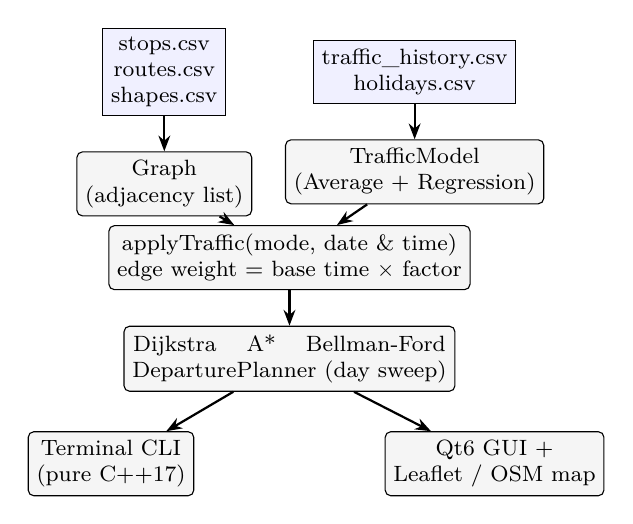
\begin{tikzpicture}[
  font=\footnotesize,
  box/.style={draw, rounded corners=2pt, align=center, minimum height=0.8cm, inner sep=3pt, fill=gray!8},
  data/.style={draw, align=center, minimum height=0.7cm, inner sep=3pt, fill=blue!6},
  arr/.style={-{Stealth[length=2mm]}, thick},
  node distance=0.45cm and 0.35cm]
  \node[data] (stops) {stops.csv\\routes.csv\\shapes.csv};
  \node[data, right=1.1cm of stops] (hist) {traffic\_history.csv\\holidays.csv};
  \node[box, below=of stops] (graph) {Graph\\(adjacency list)};
  \node[box, below=of hist] (tm) {TrafficModel\\(Average + Regression)};
  \node[box, below=0.6cm of $(graph)!0.5!(tm)$] (apply) {applyTraffic(mode, date \& time)\\edge weight = base time $\times$ factor};
  \node[box, below=of apply] (algos) {Dijkstra \quad A* \quad Bellman-Ford\\DeparturePlanner (day sweep)};
  \node[box, below left=0.5cm and -0.9cm of algos] (cli) {Terminal CLI\\(pure C++17)};
  \node[box, below right=0.5cm and -0.9cm of algos] (gui) {Qt6 GUI +\\Leaflet / OSM map};
  \draw[arr] (stops) -- (graph);
  \draw[arr] (hist) -- (tm);
  \draw[arr] (graph) -- (apply);
  \draw[arr] (tm) -- (apply);
  \draw[arr] (apply) -- (algos);
  \draw[arr] (algos) -- (cli);
  \draw[arr] (algos) -- (gui);
\end{tikzpicture}
\caption{System architecture. The traffic model only changes edge weights; the routing algorithms are unchanged.}
\label{fig:arch}
\end{figure}

\subsection{Transit Network}
The network contains 24 hubs (vertices) with latitude and longitude,
including Swargate, Shivajinagar, Pune Railway Station, Hinjewadi Phase~3,
Kharadi and Katraj. They are joined by 38 bidirectional corridors, stored
as 76 directed edges. Each corridor records its length in kilometres, a
free-flow travel time in minutes, the road name, and a \emph{road type}.
Road types group corridors with similar traffic behaviour
(Table~\ref{tab:data}). A separate shapes file supplies polyline
coordinates so that routes follow real roads on the map.

\begin{table}[t]
\caption{Dataset Summary}
\label{tab:data}
\centering
\begin{tabular}{@{}lr@{}}
\toprule
Item & Value \\
\midrule
Transit hubs (vertices) & 24 \\
Corridors / directed edges & 38 / 76 \\
\quad IT corridor & 5 \\
\quad City centre & 11 \\
\quad Arterial & 15 \\
\quad Highway & 7 \\
Traffic observations (2025, 150 days) & 14{,}400 \\
\quad Training / test rows (80/20) & 11{,}520 / 2{,}880 \\
Holidays and festivals listed (2025--2027) & 28 \\
\bottomrule
\end{tabular}
\end{table}

\subsection{Traffic History}
Hourly traffic data for Pune is not publicly available, so the traffic
history is \textbf{synthetic}. A short Python script using only the
standard library generates 150 randomly chosen days of 2025, with one
row per day, hour and road type. Each row stores the \emph{congestion
factor}
\begin{equation}
  c = \frac{\text{actual travel time}}{\text{free-flow travel time}} \ge 1 .
\end{equation}
The generator encodes well-known local patterns: smooth morning
(centred at 9:30~AM) and evening (6:30~PM) peaks on working days, the
strongest peaks on IT corridors, all-day congestion in the old city,
lighter midday traffic on weekends and holidays, empty roads at night,
an additional slowdown during the monsoon (June--September), and
Gaussian noise ($\sigma=0.08$). A fixed random seed makes the file
reproducible. The pipeline accepts real data with the same four columns
(\texttt{date, hour, road\_type, congestion\_factor}) without any code
change.

% =====================================================================
\section{Routing Algorithms}\label{sec:algos}

The graph $G=(V,E)$ is stored as an adjacency list
(\texttt{unordered\_map} from stop ID to a vector of edges), which needs
$O(V+E)$ memory and is well suited to this sparse network
($E \approx 3V$). Every algorithm minimises a generic edge cost
$w(e)$, which is either the distance in kilometres or the predicted
travel time in minutes (Section~\ref{sec:tdrouting}).

\subsection{Dijkstra's Algorithm (Greedy)}
A min-heap (\texttt{std::priority\_queue}) holds (tentative cost, vertex)
pairs. The vertex with the smallest cost is settled and its outgoing
edges are relaxed: if $d[u]+w(u,v) < d[v]$, then $d[v]$ is updated and
$v$ is pushed. The search stops as soon as the target is settled.

\subsection{A* Search (Informed)}
A* orders the heap by $f(n)=g(n)+h(n)$, where $g$ is the cost so far.
In distance mode, $h(n)$ is the great-circle (Haversine)
distance~\cite{sinnott1984} to the target,
\begin{equation}
  h(n) = 2R \arcsin\!\sqrt{\sin^2\!\tfrac{\Delta\phi}{2} + \cos\phi_1\cos\phi_2 \sin^2\!\tfrac{\Delta\lambda}{2}},
\end{equation}
with $R=6371$~km, $\phi$ the latitude and $\lambda$ the longitude. No road
can be shorter than the straight line between its ends, so $h$ is
admissible and consistent.

\subsection{Bellman-Ford (Dynamic Programming)}
Bellman-Ford relaxes the full edge list up to $|V|-1$ times. We stop
early when a pass makes no update, and run one extra pass to detect
negative cycles. The network has no negative weights, but the
implementation demonstrates the dynamic-programming paradigm and serves
as an independent correctness check for the other two algorithms.

\begin{table}[t]
\caption{Algorithm Characteristics}
\label{tab:complexity}
\centering
\begin{tabular}{@{}llll@{}}
\toprule
Algorithm & Paradigm & Time & Space \\
\midrule
Dijkstra     & Greedy            & $O((V+E)\log V)$ & $O(V)$ \\
A* search    & Heuristic         & $O((V+E)\log V)$ & $O(V)$ \\
Bellman-Ford & Dyn.\ programming & $O(V\cdot E)$    & $O(V)$ \\
\bottomrule
\end{tabular}
\end{table}

% =====================================================================
\section{Traffic Prediction}\label{sec:traffic}

The task is to predict the congestion factor $\hat{c}$ for a road type
$r$ at a date and time $t$. Each date is classified as a
\emph{weekday}, \emph{weekend} or \emph{holiday} (using the holiday file).
The day of the week is computed with Sakamoto's method, so no date
library is needed. Every fifth row of the history is held out for
testing, giving an 80/20 split.

\subsection{Model A: Historical Average}
Training rows are grouped by the key (road type, day type, hour), and
the prediction is the mean factor of the matching group:
\begin{equation}
  \hat{c}_{\text{avg}}(r,t) = \frac{1}{|S_k|}\sum_{i\in S_k} c_i ,
\end{equation}
where $S_k$ is the set of training rows with key
$k=(r,\ \text{daytype}(t),\ \text{hour}(t))$.
This is effectively a lookup table of $4\times3\times24=288$ cells. Its
weaknesses are that it ignores any factor that is not part of the key,
such as the monsoon, and that it has nothing to say about unseen keys.

\subsection{Model B: Linear Regression}
The regression predicts $\hat{c}_{\text{lr}} = \mathbf{w}^\top\mathbf{x}$,
where $\mathbf{x}\in\{0,1\}^9$ is a vector of binary features
(Table~\ref{tab:weights}). Because every feature is either 0 or 1, each
learned weight reads directly as ``this condition adds $w_j$ to the
congestion factor.'' The interaction terms (rush hour combined with a
road type) let IT corridors peak more sharply than highways.

The weights minimise the mean squared error over the $N$ training rows,
\begin{equation}
  J(\mathbf{w}) = \frac{1}{2N}\sum_{i=1}^{N}\left(\mathbf{w}^\top\mathbf{x}_i - c_i\right)^2,
\end{equation}
using full-batch gradient descent (Algorithm~\ref{alg:gd}) with learning
rate $\eta=0.5$ for 1000 epochs. We checked convergence against a 5000-epoch run, where
every weight agreed to within $0.002$. Training takes about
0.25~s at start-up.

\begin{algorithm}[t]
\caption{Batch Gradient Descent for the Congestion Model}
\label{alg:gd}
\begin{algorithmic}[1]
\Require training rows $(\mathbf{x}_i, c_i)$, $i=1..N$; rate $\eta$; epochs $T$
\State $\mathbf{w} \gets \mathbf{0}$
\For{$\text{epoch} = 1$ \textbf{to} $T$}
  \State $\mathbf{g} \gets \mathbf{0}$
  \For{$i = 1$ \textbf{to} $N$}
    \State $e \gets \mathbf{w}^\top \mathbf{x}_i - c_i$ \Comment{prediction error}
    \State $\mathbf{g} \gets \mathbf{g} + e\,\mathbf{x}_i$
  \EndFor
  \State $\mathbf{w} \gets \mathbf{w} - \eta\,\mathbf{g}/N$
\EndFor
\State \Return $\mathbf{w}$
\end{algorithmic}
\end{algorithm}

\begin{table}[t]
\caption{Learned Regression Weights}
\label{tab:weights}
\centering
\begin{tabular}{@{}lr@{}}
\toprule
Feature (0 or 1) & Weight \\
\midrule
Bias (always 1)                      & $+1.011$ \\
Daytime (6~AM--10~PM)                & $+0.149$ \\
Weekday morning rush (8--11~AM)      & $+0.441$ \\
Weekday evening rush (5--9~PM)       & $+0.419$ \\
Rush hour \textbf{and} IT corridor   & $+0.502$ \\
Rush hour \textbf{and} city centre   & $+0.148$ \\
Rush hour \textbf{and} highway       & $-0.338$ \\
City-centre road (daytime)           & $+0.200$ \\
Monsoon month (June--September)      & $+0.148$ \\
\bottomrule
\end{tabular}
\end{table}

For example, an IT corridor at 9:00~AM on a working day in November
gives $1.011+0.149+0.441+0.502 = 2.10$, i.e., a trip takes about twice
as long as on an empty road.

\subsection{Clamping}
Both models' outputs are clamped to $[1.0,\,4.0]$. The lower bound
encodes the physical fact that traffic can only slow a road down, which
is also what keeps the time-based A* heuristic admissible
(Section~\ref{sec:tdrouting}).

\subsection{Accuracy}
Table~\ref{tab:accuracy} reports the mean absolute error (MAE) on the
2{,}880 unseen test rows. Both models cut the error of the no-traffic
baseline substantially, by $2.8\times$ (regression) and $4.0\times$ (average). The historical average is
the more accurate of the two, because it fits every hour separately,
while the regression only knows coarse rush-hour windows. The regression
compresses the same information into nine readable numbers and is the
only one of the two that captures the monsoon. In July at 9:00~AM it
predicts $2.25$ for IT corridors versus $2.10$ in November, whereas the
lookup table returns $2.58$ in both months.

\begin{table}[t]
\caption{Prediction Error on the Held-Out Test Set}
\label{tab:accuracy}
\centering
\begin{tabular}{@{}lcc@{}}
\toprule
Model & MAE & $R^2$ \\
\midrule
No traffic (always 1.0)  & 0.328 & -- \\
Historical average       & \textbf{0.083} & -- \\
Linear regression (GD)   & 0.117 & 0.79 \\
\bottomrule
\end{tabular}
\end{table}

% =====================================================================
\section{Traffic-Aware Routing}\label{sec:tdrouting}

\subsection{Edge Weights}
For a departure time $t$, every edge receives
\begin{equation}
  w_t(e) = \tau_0(e)\cdot \hat{c}\big(r(e),\,t\big),
\end{equation}
where $\tau_0(e)$ is the free-flow time and $r(e)$ the road type. All
three algorithms then run \emph{unchanged} on these minutes instead of
kilometres. Since $w_t(e) > 0$, Dijkstra remains correct.

\subsection{Admissible Time Heuristic for A*}
A distance heuristic is not comparable with minutes. We therefore divide
the Haversine distance by the fastest free-flow speed on the network,
\begin{equation}
  h_t(n) = \frac{60 \cdot h(n)}{v_{\max}},\qquad
  v_{\max} = \max_{e\in E}\frac{\ell(e)}{\tau_0(e)/60},
\end{equation}
where $\ell(e)$ is the edge length. Here $v_{\max}=40.5$~km/h (the Katraj
to Chandani Chowk western bypass). Any path $P$ from $n$ to the target
has length at least $h(n)$ and travel time
$\sum_{e\in P}\tau_0(e)\,\hat{c}(e) \ge \sum_{e\in P}\ell(e)/v_{\max}
\ge h(n)/v_{\max}$, because $\hat{c}\ge 1$. Hence $h_t$ never
over-estimates and A* stays optimal.

\subsection{Best Time to Leave}
The departure planner sweeps the chosen day in 30-minute slots from
5:00~AM to 11:30~PM. For each slot it predicts the edge weights, runs
Dijkstra in time mode and records the fastest travel time. The slot with
the minimum is recommended. With 38 slots and sub-millisecond searches,
the whole sweep takes only a few milliseconds.

% =====================================================================
\section{Implementation}\label{sec:impl}

The core is written in standard C++17 with no external libraries. It
uses only the standard library: a priority queue for the heaps, hash
maps for the graph, and \texttt{<chrono>} for microsecond timing. Each
algorithm lives in its own
\texttt{.h/.cpp} pair, and \texttt{TrafficModel} and
\texttt{DeparturePlanner} add about 350 lines. The terminal client builds
with a single \texttt{g++} command and accepts a departure time
(\texttt{--at}), a model choice (\texttt{--model}), a day sweep
(\texttt{--best-departure}) and a model summary (\texttt{--model-info}). The desktop client
uses Qt6 Widgets~\cite{qt6} with an embedded web view that runs
Leaflet~\cite{leaflet} on OpenStreetMap~\cite{osm} tiles. A Qt WebChannel
bridge sends the network, the route and per-edge congestion factors to
JavaScript, which colours each road green ($<1.3$), yellow
($1.3$--$1.8$) or red ($>1.8$). A departure date-time picker, a
traffic-model selector and a bar chart of the day sweep complete the
interface. Continuous integration on GitHub Actions builds the CLI and
runs both distance-mode and traffic-mode queries on every push.

% =====================================================================
\section{Results}\label{sec:results}

All timings are medians of 501 runs on an AMD Ryzen~7 5700U laptop
(GCC~16, \texttt{-O2}). They measure only the search loop, not path
reconstruction.

\subsection{Algorithm Comparison}
Table~\ref{tab:bench} compares the algorithms on five representative
trips. In every case all three return identical costs and identical
paths, which cross-validates the implementations. In distance mode A*
explores far fewer vertices than Dijkstra, e.g., 5 versus 21 for Nigdi to
Kharadi, because the Haversine heuristic is tight on this geographically
spread network. Bellman-Ford's work, counted as passes $\times\,|V|$, is
between 2 and 24 times higher, matching its $O(V\cdot E)$ bound.

\begin{table*}[t]
\caption{Algorithm Benchmarks (D = Dijkstra, A = A*, B = Bellman-Ford). Traffic mode uses linear regression, Wednesday 18 Nov 2026, 9:00~AM.}
\label{tab:bench}
\centering
\footnotesize
\setlength{\tabcolsep}{3.2pt}
\begin{tabular}{@{}l|cc|ccc|ccc||cc|ccc|ccc@{}}
\toprule
& \multicolumn{8}{c||}{Distance mode (no traffic)} & \multicolumn{8}{c}{Traffic mode (fastest time)} \\
Trip & km & min & \multicolumn{3}{c|}{Nodes (D/A/B)} & \multicolumn{3}{c||}{Time $\mu$s (D/A/B)} & km & min & \multicolumn{3}{c|}{Nodes (D/A/B)} & \multicolumn{3}{c}{Time $\mu$s (D/A/B)} \\
\midrule
Swargate $\to$ Hinjewadi Ph.~3 & 26.4 & 93  & 24 & 16 & 192 & 43 & 46 & 154 & 30.2 & 122.3 & 24 & 23 & 192 & 43 & 54 & 156 \\
Kothrud $\to$ Swargate         & 7.7  & 30  & 6  & 3  & 144 & 16 & 16 & 122 & 13.8 & 56.9  & 10 & 9  & 144 & 24 & 29 & 124 \\
Nigdi $\to$ Kharadi            & 28.2 & 69  & 21 & 5  & 120 & 40 & 21 & 104 & 28.2 & 116.5 & 23 & 21 & 120 & 25 & 31 & 72 \\
Katraj $\to$ Viman Nagar       & 18.1 & 60  & 18 & 8  & 144 & 35 & 31 & 116 & 18.1 & 100.9 & 23 & 22 & 144 & 27 & 33 & 76 \\
Hinjewadi Ph.~3 $\to$ Hadapsar & 31.6 & 104 & 21 & 11 & 48  & 38 & 34 & 63  & 41.8 & 144.9 & 20 & 17 & 96  & 23 & 28 & 66 \\
\bottomrule
\end{tabular}
\end{table*}

In traffic mode the advantage of A* largely disappears (for example, 23
versus 24 nodes for Swargate to Hinjewadi). The time heuristic assumes
the best-case speed of 40.5~km/h everywhere, while congested roads at
rush hour average far less, so $h_t$ is loose and prunes little. The
heuristic is still correct, only weaker. This illustrates a general
trade-off between admissibility and heuristic strength.

\subsection{Routes That Change With Time}
Table~\ref{tab:change} shows trips where the optimal route changes
between 2:00~PM and 9:00~AM on a weekday. At rush hour the regression
predicts city-centre roads to be about $1.95\times$ slower but highways
only $1.26\times$, so a longer bypass becomes faster. For Aundh to
Swargate, the 27.1~km western loop saves 4.8~min over the 11.5~km
city route. The savings are modest because the city route remains
competitive, but they show the routing responding correctly to the
predicted conditions.

\begin{table}[t]
\caption{Route Change Between Off-Peak and Rush Hour (Linear Regression, Weekday)}
\label{tab:change}
\centering
\footnotesize
\setlength{\tabcolsep}{3pt}
\begin{tabular}{@{}lcc@{}}
\toprule
 & Kothrud $\to$ Swargate & Aundh $\to$ Swargate \\
\midrule
Best route, 2~PM         & via Deccan        & via SPPU, Shivajinagar \\
\quad length, time       & 7.7~km, 40.8~min  & 11.5~km, 67.9~min \\
Same route, 9~AM         & 58.5~min          & 96.5~min \\
Best route, 9~AM         & via Chandani Ch., Warje & via Wakad, Warje \\
\quad length, time       & 13.8~km, 56.9~min & 27.1~km, 91.7~min \\
Saving by rerouting      & 1.6~min           & 4.8~min \\
\bottomrule
\end{tabular}
\end{table}

\subsection{Best Time to Leave}
Fig.~\ref{fig:sweep} plots the predicted Swargate to Hinjewadi Phase~3
travel time for every departure slot on a weekday. Both models agree on
the overall shape: about 75~min early in the morning and late at night,
rising to 122--142~min in the rush hours. The regression produces flat
steps because its rush-hour features are on/off windows, whereas the
historical average follows the smoother hourly profile of the data. Both
recommend leaving at 5:00~AM, or after 11:00~PM, which saves about
47--64~min compared with the worst slot.

\begin{figure}[t]
\centering
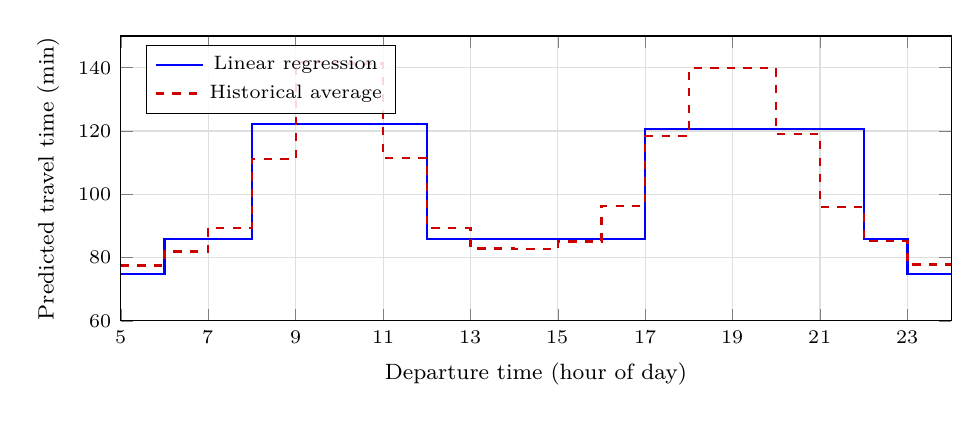
\begin{tikzpicture}
\begin{axis}[
  width=\columnwidth, height=5.2cm,
  xlabel={Departure time (hour of day)},
  ylabel={Predicted travel time (min)},
  xmin=5, xmax=24, ymin=60, ymax=150,
  xtick={5,7,9,11,13,15,17,19,21,23},
  grid=major, grid style={gray!25},
  legend pos=north west, legend style={font=\scriptsize, fill=white, fill opacity=0.85, text opacity=1},
  tick label style={font=\scriptsize}, label style={font=\footnotesize}]
\addplot[const plot, thick, blue] coordinates {
(5,74.8)(5.5,74.8)(6,85.8)(6.5,85.8)(7,85.8)(7.5,85.8)(8,122.3)(8.5,122.3)(9,122.3)(9.5,122.3)(10,122.3)(10.5,122.3)(11,122.3)(11.5,122.3)(12,85.8)(12.5,85.8)(13,85.8)(13.5,85.8)(14,85.8)(14.5,85.8)(15,85.8)(15.5,85.8)(16,85.8)(16.5,85.8)(17,120.7)(17.5,120.7)(18,120.7)(18.5,120.7)(19,120.7)(19.5,120.7)(20,120.7)(20.5,120.7)(21,120.7)(21.5,120.7)(22,85.8)(22.5,85.8)(23,74.8)(23.5,74.8)(24,74.8)};
\addlegendentry{Linear regression}
\addplot[const plot, thick, red!80!black, dashed] coordinates {
(5,77.5)(5.5,77.5)(6,81.9)(6.5,81.9)(7,89.4)(7.5,89.4)(8,111.1)(8.5,111.1)(9,141.9)(9.5,141.9)(10,141.3)(10.5,141.3)(11,111.4)(11.5,111.4)(12,89.3)(12.5,89.3)(13,82.9)(13.5,82.9)(14,82.6)(14.5,82.6)(15,85.1)(15.5,85.1)(16,96.4)(16.5,96.4)(17,118.5)(17.5,118.5)(18,139.9)(18.5,139.9)(19,139.9)(19.5,139.9)(20,119.0)(20.5,119.0)(21,96.1)(21.5,96.1)(22,85.2)(22.5,85.2)(23,77.8)(23.5,77.8)(24,77.8)};
\addlegendentry{Historical average}
\end{axis}
\end{tikzpicture}
\caption{Predicted Swargate $\to$ Hinjewadi Phase~3 travel time by departure slot, Wednesday 18 Nov 2026.}
\label{fig:sweep}
\end{figure}

\subsection{Performance}
Every single query completes in under 160~$\mu$s, including
Bellman-Ford. Training both traffic models at start-up takes about
0.25~s, and a full-day sweep of 38 Dijkstra runs takes a few
milliseconds. The system is therefore fully interactive even on modest
laboratory hardware.

% =====================================================================
\section{Limitations and Future Work}\label{sec:limits}

\begin{itemize}
  \item \textbf{Synthetic data.} The traffic history is generated, not
        measured. The results demonstrate the method, not real Pune
        accuracy. Replacing the CSV with real probe or sensor data is
        the most valuable next step.
  \item \textbf{Static snapshot.} Congestion is predicted once at the
        departure time and applied to the whole trip. A true
        time-dependent search would evaluate each edge at the time the
        bus reaches it~\cite{cooke1966,kaufman1993}. This would require
        smoothing the hourly factors so that FIFO holds.
  \item \textbf{Road-level, not bus-level.} The model ignores
        timetables, waiting and transfer times, and bus capacity.
  \item \textbf{Model capacity.} Finer hourly features or a small
        tree-based model could close the gap to the historical average
        while keeping the model readable.
  \item \textbf{Heuristic strength.} A tighter time heuristic, e.g.,
        landmark-based lower bounds~\cite{delling2009}, would restore
        A*'s pruning advantage in traffic mode.
\end{itemize}

% =====================================================================
\section{Conclusion}\label{sec:conclusion}

We presented a compact, fully explainable route optimizer for Pune's
PMPML network that combines three classical shortest-path paradigms
with date- and time-aware congestion prediction. Both prediction models
reduce the no-traffic error by a factor of 2.8 to 4. Because the
predicted factors are applied only to the edge weights, the textbook
algorithms remain untouched and provably correct. A single admissible
heuristic change keeps A* optimal in time mode. The system changes
routes at rush hour, recommends the best departure time and answers
every query in microseconds. It shows that a meaningful machine learning
component can be added to an algorithms project without giving up
transparency.

% =====================================================================
\begin{thebibliography}{99}

\bibitem{dijkstra1959}
E.~W. Dijkstra, ``A note on two problems in connexion with graphs,''
\emph{Numerische Mathematik}, vol.~1, pp.~269--271, 1959.

\bibitem{hart1968}
P.~E. Hart, N.~J. Nilsson, and B.~Raphael, ``A formal basis for the
heuristic determination of minimum cost paths,'' \emph{IEEE Trans. Syst.
Sci. Cybern.}, vol.~4, no.~2, pp.~100--107, Jul. 1968.

\bibitem{bellman1958}
R.~Bellman, ``On a routing problem,'' \emph{Quart. Appl. Math.},
vol.~16, no.~1, pp.~87--90, 1958.

\bibitem{ford1956}
L.~R. Ford, Jr., ``Network flow theory,'' RAND Corp., Santa Monica, CA,
USA, Paper P-923, 1956.

\bibitem{clrs}
T.~H. Cormen, C.~E. Leiserson, R.~L. Rivest, and C.~Stein,
\emph{Introduction to Algorithms}, 3rd~ed. Cambridge, MA, USA: MIT Press,
2009.

\bibitem{delling2009}
D.~Delling, P.~Sanders, D.~Schultes, and D.~Wagner, ``Engineering route
planning algorithms,'' in \emph{Algorithmics of Large and Complex
Networks} (LNCS, vol.~5515). Berlin, Germany: Springer, 2009,
pp.~117--139.

\bibitem{cooke1966}
K.~L. Cooke and E.~Halsey, ``The shortest route through a network with
time-dependent internodal transit times,'' \emph{J. Math. Anal. Appl.},
vol.~14, no.~3, pp.~493--498, 1966.

\bibitem{dreyfus1969}
S.~E. Dreyfus, ``An appraisal of some shortest-path algorithms,''
\emph{Oper. Res.}, vol.~17, no.~3, pp.~395--412, 1969.

\bibitem{kaufman1993}
D.~E. Kaufman and R.~L. Smith, ``Fastest paths in time-dependent networks
for intelligent vehicle-highway systems application,'' \emph{IVHS J.},
vol.~1, no.~1, pp.~1--11, 1993.

\bibitem{williams2003}
B.~M. Williams and L.~A. Hoel, ``Modeling and forecasting vehicular
traffic flow as a seasonal ARIMA process: Theoretical basis and
empirical results,'' \emph{J. Transp. Eng.}, vol.~129, no.~6,
pp.~664--672, 2003.

\bibitem{lv2015}
Y.~Lv, Y.~Duan, W.~Kang, Z.~Li, and F.-Y. Wang, ``Traffic flow prediction
with big data: A deep learning approach,'' \emph{IEEE Trans. Intell.
Transp. Syst.}, vol.~16, no.~2, pp.~865--873, Apr. 2015.

\bibitem{hastie2009}
T.~Hastie, R.~Tibshirani, and J.~Friedman, \emph{The Elements of
Statistical Learning}, 2nd~ed. New York, NY, USA: Springer, 2009.

\bibitem{sinnott1984}
R.~W. Sinnott, ``Virtues of the haversine,'' \emph{Sky and Telescope},
vol.~68, no.~2, p.~159, 1984.

\bibitem{osm}
M.~Haklay and P.~Weber, ``OpenStreetMap: User-generated street maps,''
\emph{IEEE Pervasive Comput.}, vol.~7, no.~4, pp.~12--18, Oct.--Dec. 2008.

\bibitem{leaflet}
V.~Agafonkin, ``Leaflet: An open-source JavaScript library for
interactive maps,'' 2024. [Online]. Available: \url{https://leafletjs.com}

\bibitem{qt6}
The Qt Company, ``Qt 6 documentation,'' 2024. [Online]. Available:
\url{https://doc.qt.io/qt-6/}

\end{thebibliography}

\end{document}
